\chapter{Simulation Preparation} \label{chap:Simulation Preparation}
This chapter introduces the system modeling process for preparing the state estimation simulation. During the system modeling section, the topology of the system is built based on a 400V IEEE European test system with 206 buses and 205 branches, and pseudo-measurements are generated to ensure the observability of the system. There are totally 30 scenarios generated for different levels of measurements, where each scenario contains 100 cases with different locations of installed smart meters, distributed by Monta-Carlo simulation. After the modeling of the system, the four state estimation algorithms introduced in Chapter \ref{chap:Math_for} are implemented and tested on this system.

\section{Introduction of Test System}
The test system is a distribution grid with a radial topology. In this project, this system is assumed to be balanced, and the single phase model is used during the simulation. The feeder bus is defined as the slack bus and the base power is set to 1000 VA. Because the distribution grid branches have shorter distance and smaller diameter than the transmission grid, the distribution grid has a high $R/X$ ratio and small line-to-ground capacitance. Thus, the line-to-ground capacitance of the tested distribution grid is assumed to be zero for simplification.
\bigskip
\\There are totally 30 tested scenarios, which can be found in Table \ref{tab:30_scenarios}, with different levels and types of measurements including bus voltage magnitude, bus injection power, and branch power flow. Smart meter measurements are available according to the following rules:
    \begin{table}[!h]
        \centering
        \begin{tabular}{c|c|c|c|c}
            Scenario Index & P Injection & Q Injection & V & Branch Power Flow \\ \hline
            $1$ & $0{\%} $ & 0{\%} & 0{\%} & 0{\%} \\
            $2$ & $0{\%} $ & 0{\%} & 0{\%} & 10{\%} \\ 
            $3$ & $0{\%} $ & 0{\%} & 0{\%} & 20{\%} \\
            $4$ & $33.3{\%} $ & 0{\%} & 0{\%} & 0{\%} \\
            $5$ & $33.3{\%} $ & 0{\%} & 0{\%} & 10{\%} \\ 
            $6$ & $33.3{\%} $ & 0{\%} & 0{\%} & 20{\%} \\
            $7$ & $33.3{\%} $ & 33.3{\%} & 0{\%} & 0{\%} \\
            $8$ & $33.3{\%} $ & 33.3{\%} & 0{\%} & 10{\%} \\ 
            $9$ & $33.3{\%} $ & 33.3{\%} & 0{\%} & 20{\%} \\
            $10$ & $33.3{\%} $ & 33.3{\%} & 33.3{\%} & 0{\%} \\
            $11$ & $33.3{\%} $ & 33.3{\%} & 33.3{\%} & 10{\%} \\ 
            $12$ & $33.3{\%} $ & 33.3{\%} & 33.3{\%} & 20{\%} \\        
            $13$ & $66.6{\%} $ & 0{\%} & 0{\%} & 0{\%} \\
            $14$ & $66.6{\%} $ & 0{\%} & 0{\%} & 10{\%} \\ 
            $15$ & $66.6{\%} $ & 0{\%} & 0{\%} & 20{\%} \\
            $16$ & $66.6{\%} $ & 66.6{\%} & 0{\%} & 0{\%} \\
            $17$ & $66.6{\%} $ & 66.6{\%} & 0{\%} & 10{\%} \\ 
            $18$ & $66.6{\%} $ & 66.6{\%} & 0{\%} & 20{\%} \\
            $19$ & $66.6{\%} $ & 66.6{\%} & 66.6{\%} & 0{\%} \\
            $20$ & $66.6{\%} $ & 66.6{\%} & 66.6{\%} & 10{\%} \\ 
            $21$ & $66.6{\%} $ & 66.6{\%} & 66.6{\%} & 20{\%} \\
            $22$ & $100{\%} $ & 0{\%} & 0{\%} & 0{\%} \\
            $23$ & $100{\%} $ & 0{\%} & 0{\%} & 10{\%} \\ 
            $24$ & $100{\%} $ & 0{\%} & 0{\%} & 20{\%} \\ 
            $25$ & $100{\%} $ & 100{\%} & 0{\%} & 0{\%} \\
            $26$ & $100{\%} $ & 100{\%} & 0{\%} & 10{\%} \\ 
            $27$ & $100{\%} $ & 100{\%} & 0{\%} & 20{\%} \\
            $28$ & $100{\%} $ & 100{\%} & 100{\%} & 0{\%} \\
            $29$ & $100{\%} $ & 100{\%} & 100{\%} & 10{\%} \\ 
            $30$ & $100{\%} $ & 100{\%} & 100{\%} & 20{\%}             
        \end{tabular}
        \caption{30 Scenarios of Measurements}
        \label{tab:30_scenarios}
    \end{table}

\begin{itemize}
    \item The voltage magnitude, voltage phase angle, active and reactive power injection at feeder bus are always known. The voltage magnitude is 1 p.u. and the voltage phase is 0 $rad$.
    \item The reactive power injection at a certain bus is only known if, and only if, the active power injection is also known. Otherwise, only the feeder bus has the information of the reactive power injection.
    \item The voltage magnitude value at a certain bus is only known if, and only if, the active and reactive power injection is also known.  Otherwise, only the information of the voltage magnitude at the feeder bus is known. 
    \item To ensure the observability of the system, pseudo-measurements must be generated when the active or reactive power injection at any bus is unknown. The details about pseudo-measurements generation are introduced in Sect.\ref{sect:pseudo-measurements}
    \item Active and reactive branch power flows are measured together. This means that if the active power flow at a certain branch is known, the information of the reactive power flow on the same branch must also be known.
    \item when determining how much percentage information of the active or reactive power injection is known, the virtual active or reactive power injection are not considered. For example, under the scenario 4 where $33 \%$ of the active power injection information is known, if there are 206 buses in the system and the active power injection of 30 buses have virtual measurements, then the information of $(206-30)\times \frac{33.3}{100} \approx 59$ active power injections are known through the real measurements by smart meters. 
    \item Due to the fact the branch power flow has two directions, there are two possible locations to measure the branch power flow for two power flow directions, from one bus to another and vice versa. Assuming there are 205 branches, $205 \times 2 \times \frac{10}{100} = 41 $ branch power flows are known under $10 {\%}$ power flow scenarios.
\end{itemize}

\section{Measurement Generation}
\subsection{Load Generation}
The original load data are collected from two sources by smart meters. One source is 1000 active power load for small household consumers and another source is 1000 active power injection from PV systems in the City of Basel. Both of them are recorded from April $1^{st}$ 2014 to July $1^{st}$ 2017 with a time interval of 15 minutes between each time step. So, there are totally 96 recorded time steps per day.
\bigskip
\\In order to populate the grid with loads in a realistic way, the following approach has been considered:
\begin{itemize}
    \item For each of the 206 buses in the LV distribution grid, 0 to 5 consumer loads are selected randomly from those 1000 consumers and aggregated together as a new load. This is motivated by the fact that there might be no consumers, a single family house or multiple flats (e.g., multi-family house) connected to a single node
    \item Because of the lack of reactive power consumption data, a constant power factor of 0.98 inductive is used.
    \item Concerning PV generation, 20 of them are selected from the 1000 PV generation profiles and distributed randomly to 20 buses in the distribution system.
\end{itemize}
In this way, the active and reactive power injection at each bus is obtained. Therefore, there are two types of buses in this case: slack bus for the feeder and PQ buses for other buses. Subsequently, a power flow calculation can be run for generating the full-knowledge situation, namely all voltage magnitudes and phase angles, active and reactive power injections, and active and reactive power flows. 
\bigskip
\\Because SVR-EKF needs an extra training set, the power flow calculation introduced above is run twice for generating the training set and the test set separately. The original data ranges from April 2014 to April 2017. The load and PV generation on the first day, which contains 96 time steps with 15 minutes time interval, is selected as the test group for all those four algorithms and noise is added to the measurements as introduced in Sect.\ref{sect:add noise}. The power injection of the training set is selected from the second to fourth day for both loads and PV generation. There is no noise added to the training group for both input and output data, which ensure the accuracy of the SVR in SVR-EKF. 
\subsection{Adding Noise to Measurements}
\label{sect:add noise}
As it is introduced in Chapter \ref{chap:Math_for}, the measurement from the smart meter is not perfect and white Gaussian noise is assumed in each measurement. In this project, a uniform noise is added on the measurements for imitate the white Gaussian noise with a zero mean and 0.01 standard deviation, assuming that inaccuracies are due to the externals environments of the smart meters and have no relationship with the type or value of the measurements. Thus, noise is generated randomly within $[-0.01,0.01]$ for each measurement at each time step which is shown in Equation \ref{eq:measurements with noise}:
\begin{align}
    meas_{noise} &= \epsilon + meas_{ideal}
    \label{eq:measurements with noise}
\end{align}
, where $meas_{noise}$ and $meas_{ideal}$ are measurements with and without noise, respectively. $\epsilon$ is the random number ranging between $-0.01$ and $0.01$ for measurement $meas_{ideal}$. Figure \ref{fig:meas_with_without_noise} gives an intuition of the bus voltage magnitude with and without noise over 96 time steps.
    \begin{figure}[!h]
        \centering
        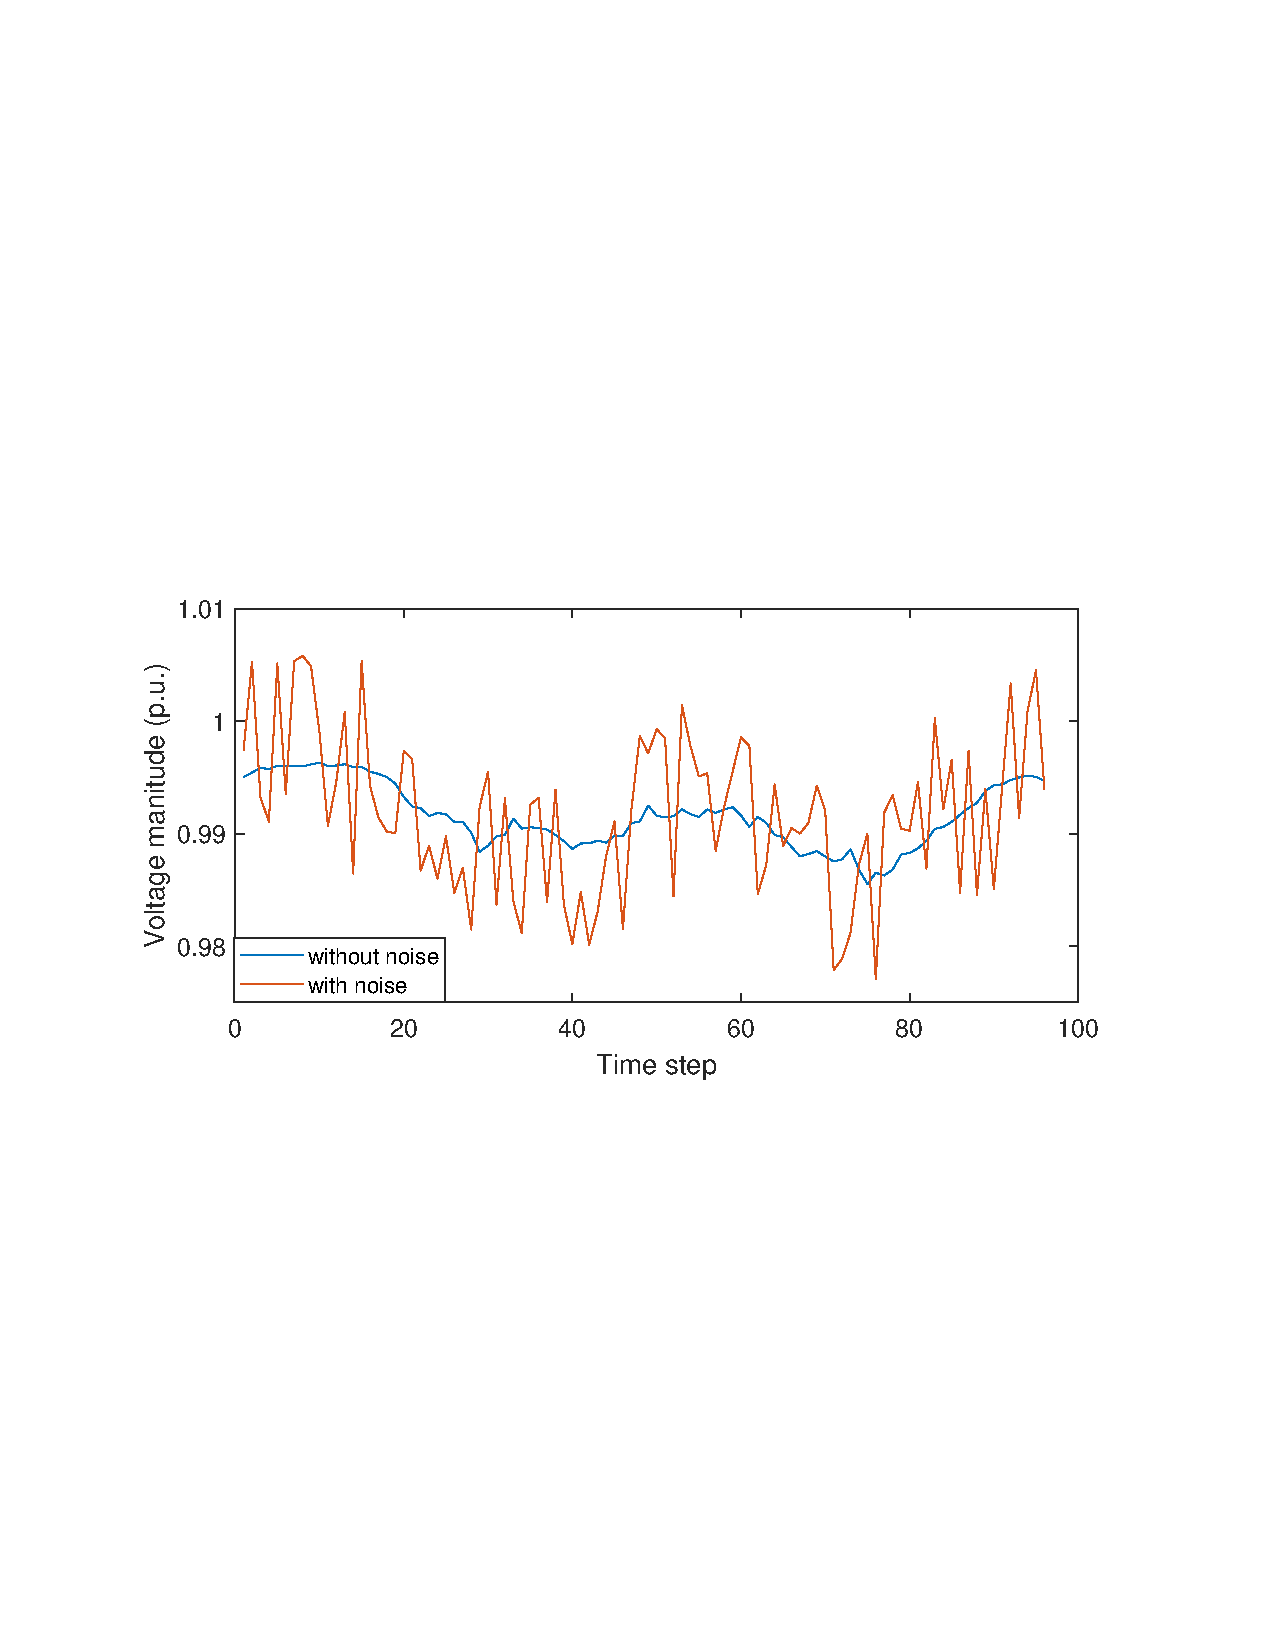
\includegraphics[ height=8cm, width=13cm]{figures/meas_with_without_noise.pdf}
        \caption{Voltage magnitude of bus 2} 
        \label{fig:meas_with_without_noise}
    \end{figure}
    
\subsection{Generation of Pseudo-Measurements}
\label{sect:pseudo-measurements}
To ensure the observability of the system, pseudo-measurements should be generated. To determine if a system is observable or not, one can easily check the rank of the measurement Jacobian matrix $H$ introduced in Equation \ref{eq:jacobian_matrix}. If the rank of the measurement Jacobian matrix is smaller than twice the number of buses, the system is unobservable. Otherwise, the system is observable. There are several existing pseudo-measurements generation methods based on machine learning skills such as SVR and ANN. This thesis generates pseudo-measurements simply based on the proportion of the total energy consumption at each bus. 
\bigskip
\\It is assumed that active and reactive power injection, and voltage magnitude and angle are known at the slack bus in all 30 scenarios.Measurements at buses without load or PV generation are defined as virtual measurements. 
\bigskip
\\The system is observable when the power injection at all buses are known in addition to the voltage magnitude and phase angle at the slack bus. Therefore, to ensure that the system is observable, all buses whose power injection is unknown, are assigned with a pseudo power injection.
\bigskip
\\Nevertheless, the total energy consumption E over the simulation period at each bus is assumed to be known, which is used to generate the pseudo power injection at buses without smart meter. In addition, knowing the active power flow at the slack bus, a measurement gap, which is called active power residual vector $p_r=[p_r^1, p_r^2,\cdots,p_r^{96}]$ for 96 time steps, is observed between this active power profile and the spatial aggregation of all active power profiles measured by smart meters, considering also PV systems as shown by Figure \ref{fig:meas_gap}.
    \begin{figure}[!h]
        \centering
        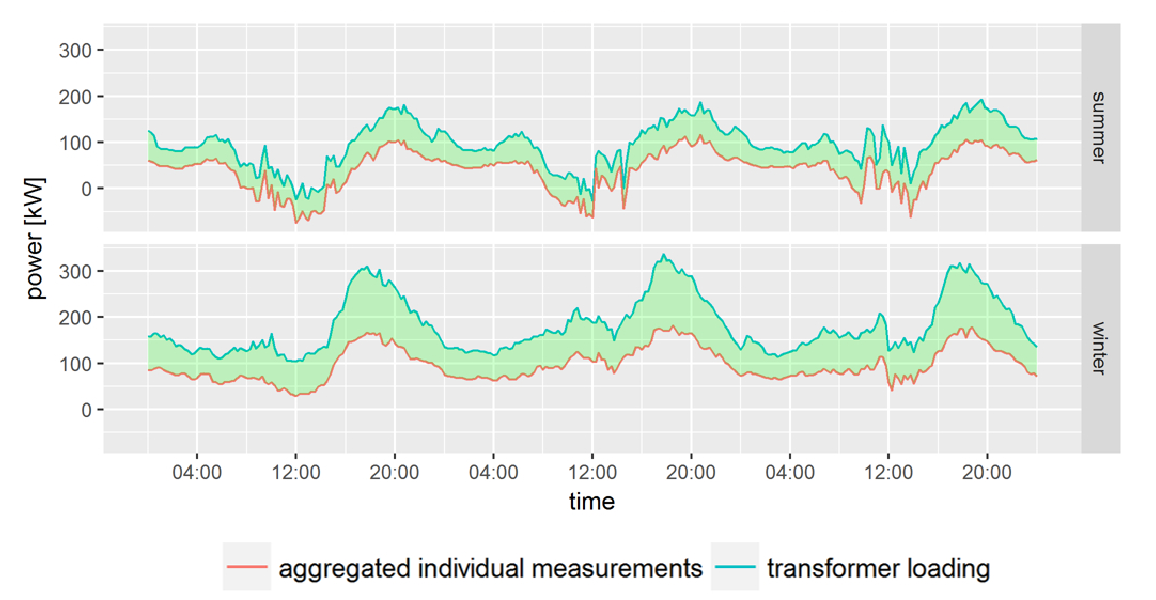
\includegraphics[ height=8.5cm, width=13cm]{figures/measurement_gap.pdf}
        \caption{Power gap between transformer loading and aggregated individual measurements} 
        \label{fig:meas_gap}
    \end{figure}
The green region is the gap corresponds to the aggregated power consumed by loads without smart meter. Pseudo-measurements of reactive power are synthesized similarly. Assuming $p_{inj}=[p_{inj}^1,p_{inj}^2,\cdots,p_{inj}^l]$ is the active power injection for $l$ buses whose active power injection is measured, and $p_{inj}^i=[p_{inj}^{i,1}, p_{inj}^{i,2},\cdots,p_{inj}^{i,96}]$ is the $i^{th}$ measured active power injection for 96 time steps. The active power gap $p_{c}$ in Figure \ref{fig:meas_gap} can be obtained as follows:
\begin{align}
    p_c &= \sum_{i=1}^{l} p_{inj}^i+\sum_{i=1}^{g} p_{gen}^i
    \label{eq:pseudo_power_injection_curve}
\end{align}
, where $p_{gen}=[p_{gen}^1,p_{gen}^2,\cdots,p_{gen}^g]$ is the active power generation from the PV generators, and $g$ is the number of PV generators which equals to 20 in this thesis. Hence, pseudo-measurements are created for each non-measured load by splitting the measurement gap profile into multiple active power profiles (i.e. one profile per non-measured load) according to their total energy consumption $E_c=[E_c^1,E_c^2,\cdots,E_c^p]$, where $p$ is the total number of buses whose active power injection is not measured \cite{ghosh1997load}. Assuming $E_c=[E_c^1,E_c^2,\cdots,E_c^p]$ is the total active energy consumption for the buses without active power measurements, and $p$ is the total number of buses who do not have active power injection information. Then, the pseudo active power consumption of the $i^{th}$  bus can be formulated as:
\begin{align}
    p_{psu-con}^{i} &= \frac{E_c^i}{\sum_{j=1}^{p}E_c^j} p_c 
    \label{eq:pseu_con}
\end{align}
, where each non-metered load is assigned with a profile of similar shape to the gap profile, but scaled to its total energy consumption as shown in Figure \ref{fig:pseudo_scale}.
    \begin{figure}[!h]
        \centering
        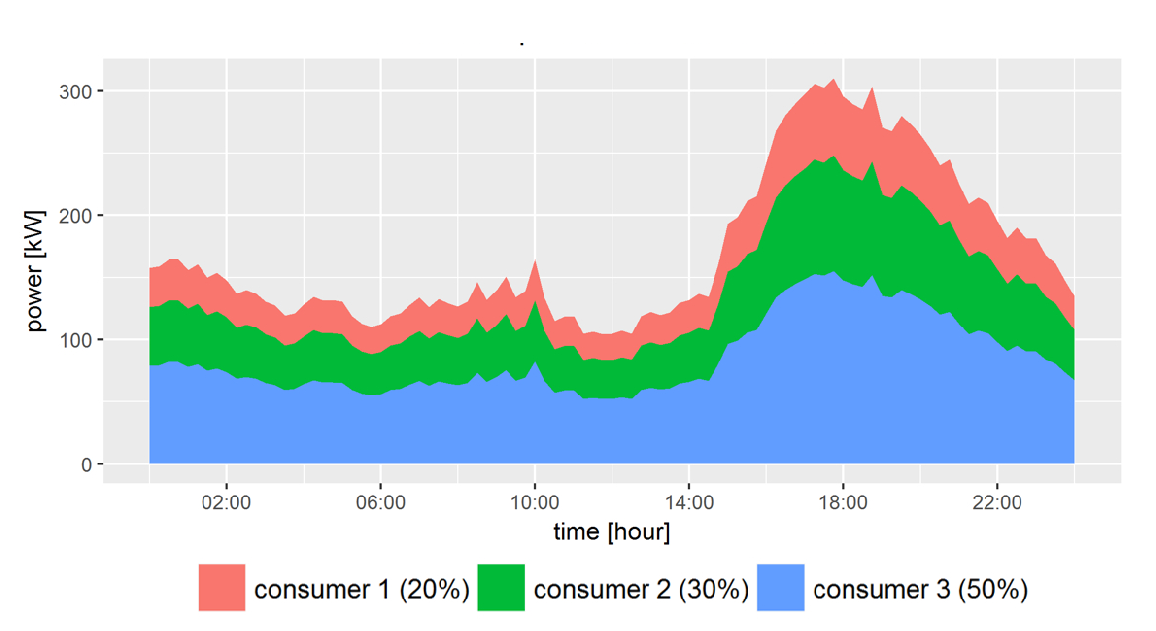
\includegraphics[ height=7.5cm, width=13cm]{figures/pseudo_measurements.pdf}
        \caption{Reference profile and load allocation}
        \label{fig:pseudo_scale}
    \end{figure}
,as for the pseudo active power injection of the bus, if there is no PV generator connected to the bus, the active power injection equals the pseudo active power consumption. Otherwise, the PV generation at that bus $p_{gen}^j$ should be added to the pseudo active power consumption to get the pseudo active power injection at bus $i$ as follows:
\begin{align}
    p_{psu}^{i} &= p_{psu-con}^{i}+p_{gen}^j
    \label{eq:pseu_inj}
\end{align}
By using the equations introduced above, the pseudo active power injections can be generated for buses without information on active power injection. The process for generating pseudo reactive power injection is similar to the pseudo active power injection generation except that there is no reactive power generation from PV generator. Because the aim of generating pseudo-measurements is to ensure the observability of the system and pseudo-measurements usually have a big mismatch to its real measured value, the standard deviation of the pseudo-measurements are set to be 0.3 p.u. which is substantially higher than the standard deviation from smart meters and virtual measurements which are set to 0.01. By using a Monta-Carlo simulation for selecting different meters locations, 100 cases are generated for each of the 30 scenarios. Figures \ref{fig:Pseudo Active Power Injection at Bus 2} and \ref{fig:Pseudo Active Power Injection at Bus 4} show two typical pseudo active power injections and its real active power injection.
    \begin{figure}[!h]
        \centering
        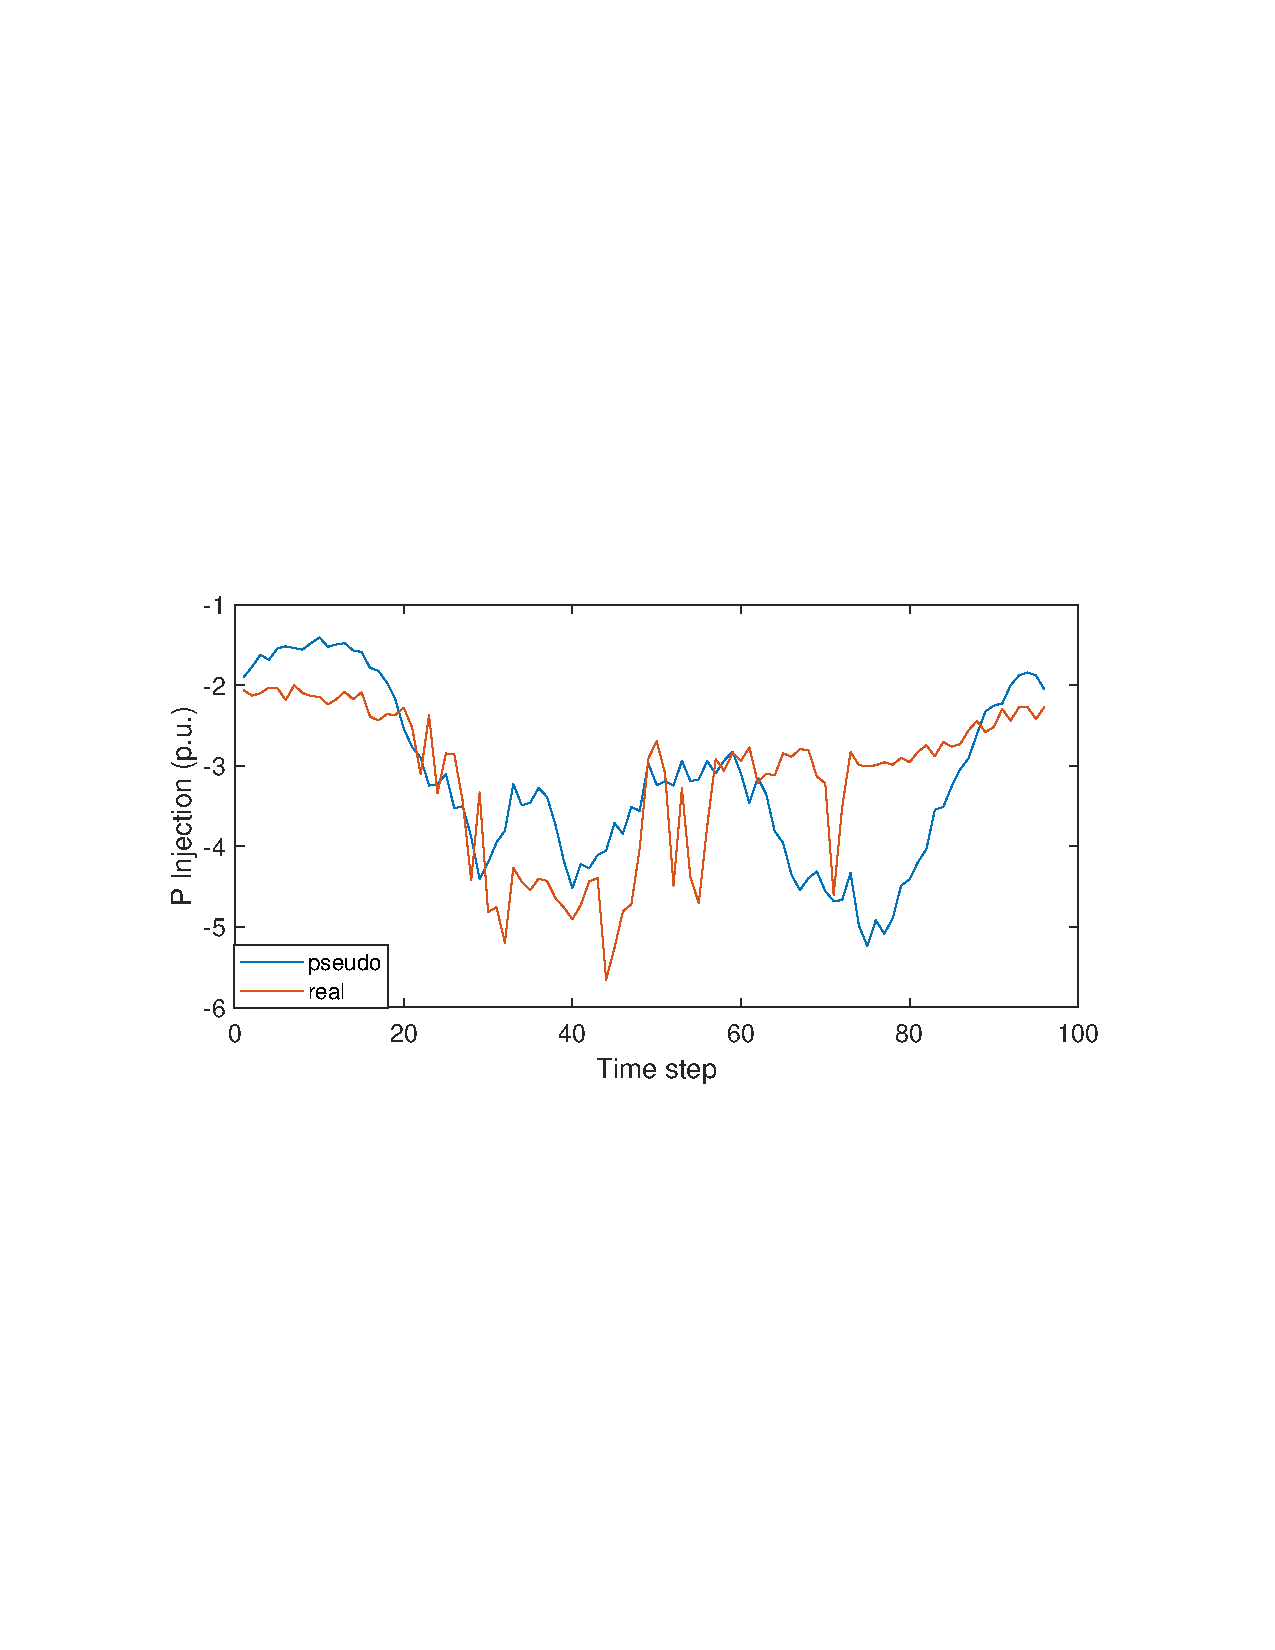
\includegraphics[ height=7cm, width=12cm]{figures/pseudo_P_1.pdf}
        \caption{Pseudo and actual active power injection}
        \label{fig:Pseudo Active Power Injection at Bus 2}
    \end{figure}
    
    \begin{figure}[!h]
        \centering
        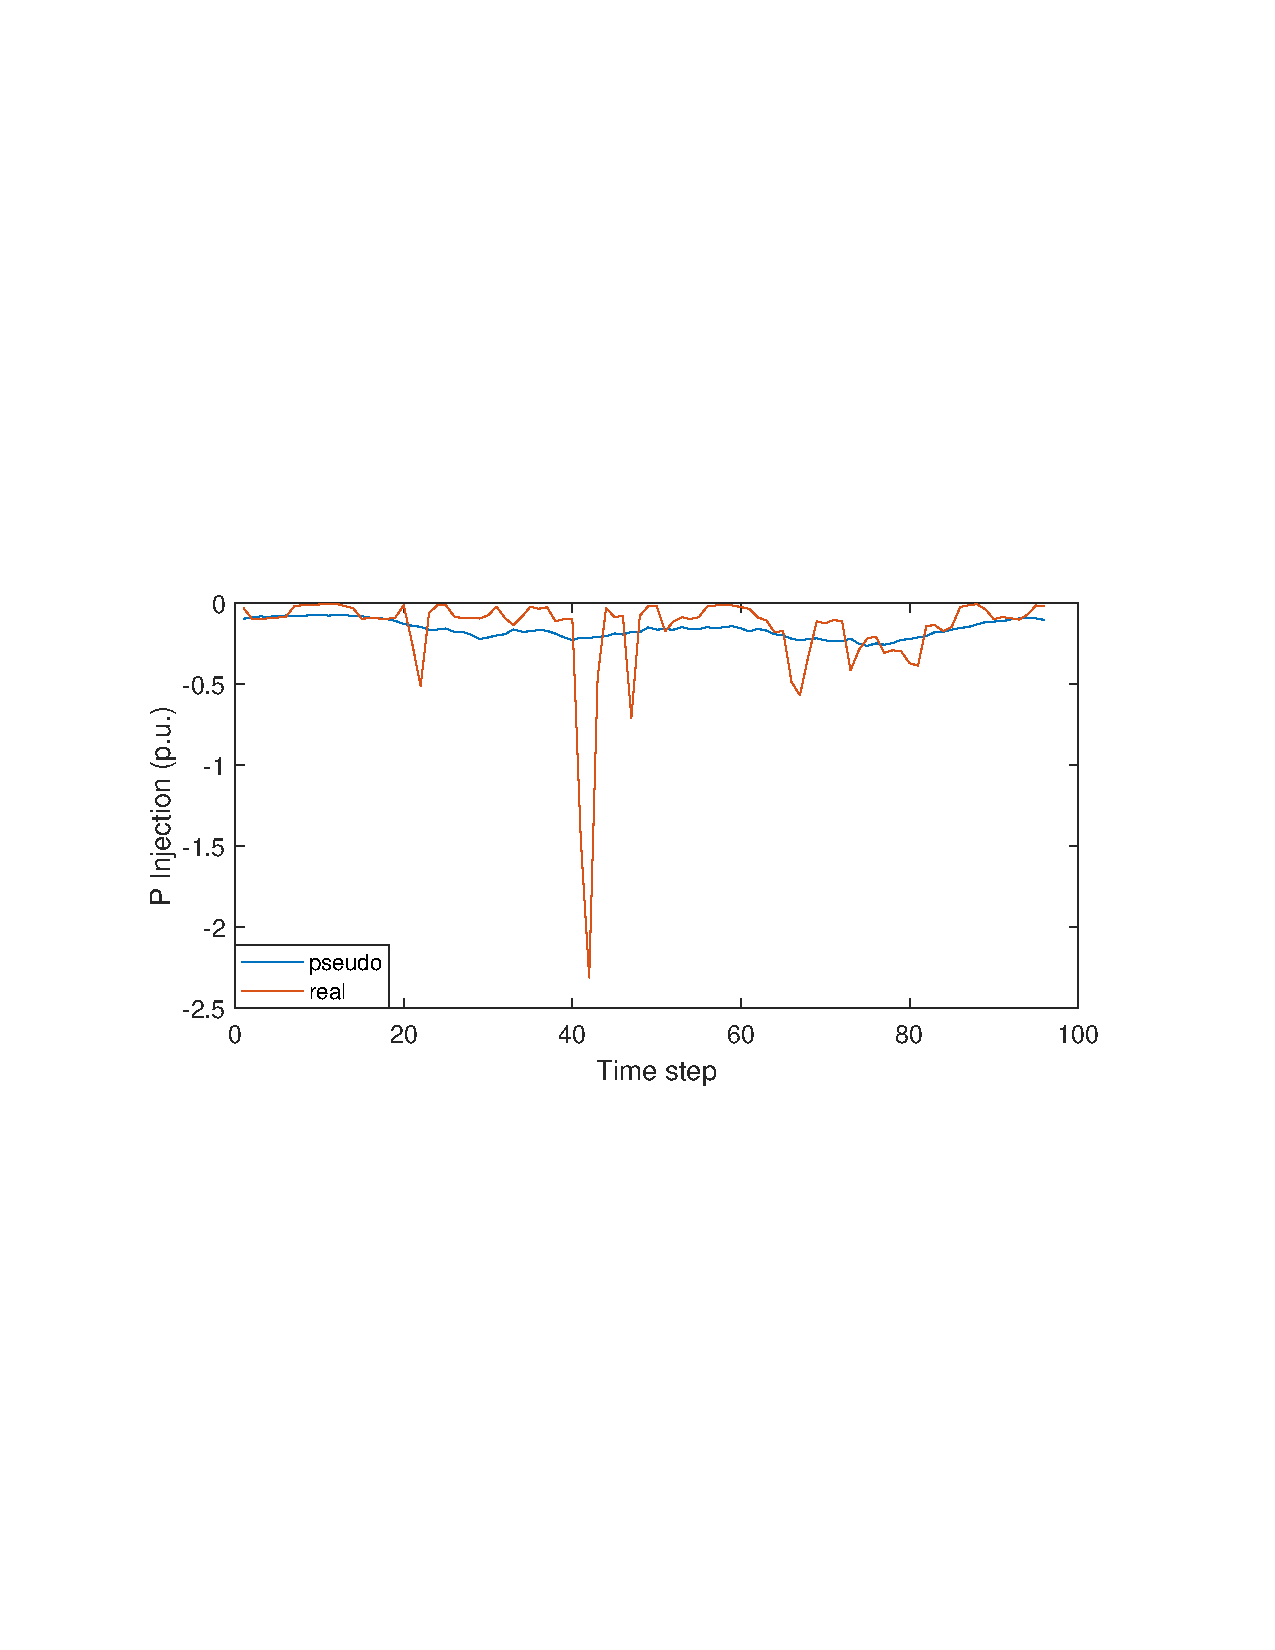
\includegraphics[ height=7cm, width=12cm]{figures/pseudo_P_2.pdf}
        \caption{Pseudo and actual active power injection} 
        \label{fig:Pseudo Active Power Injection at Bus 4}
    \end{figure}
\noindent
It can be seen that the pseudo active power injection follows the main trend of the real active power injection since the curve is relatively smooth, but the proposed pseudo-measurements generation method based on the total energy consumption can not match well when the load changes fast and sharply as shown in Figure \ref{fig:Pseudo Active Power Injection at Bus 4}, notably at time step 41, where there is a big mismatch between the pseudo measurement and its real value. However, despite the big mismatch at time step 41 in Figure \ref{fig:Pseudo Active Power Injection at Bus 4}, the overall absolute mismatch through all 96 time steps at bus 4 is smaller than the one in Figure \ref{fig:Pseudo Active Power Injection at Bus 2} due to the lower mean power level.
    \begin{figure}[!h]
        \centering
        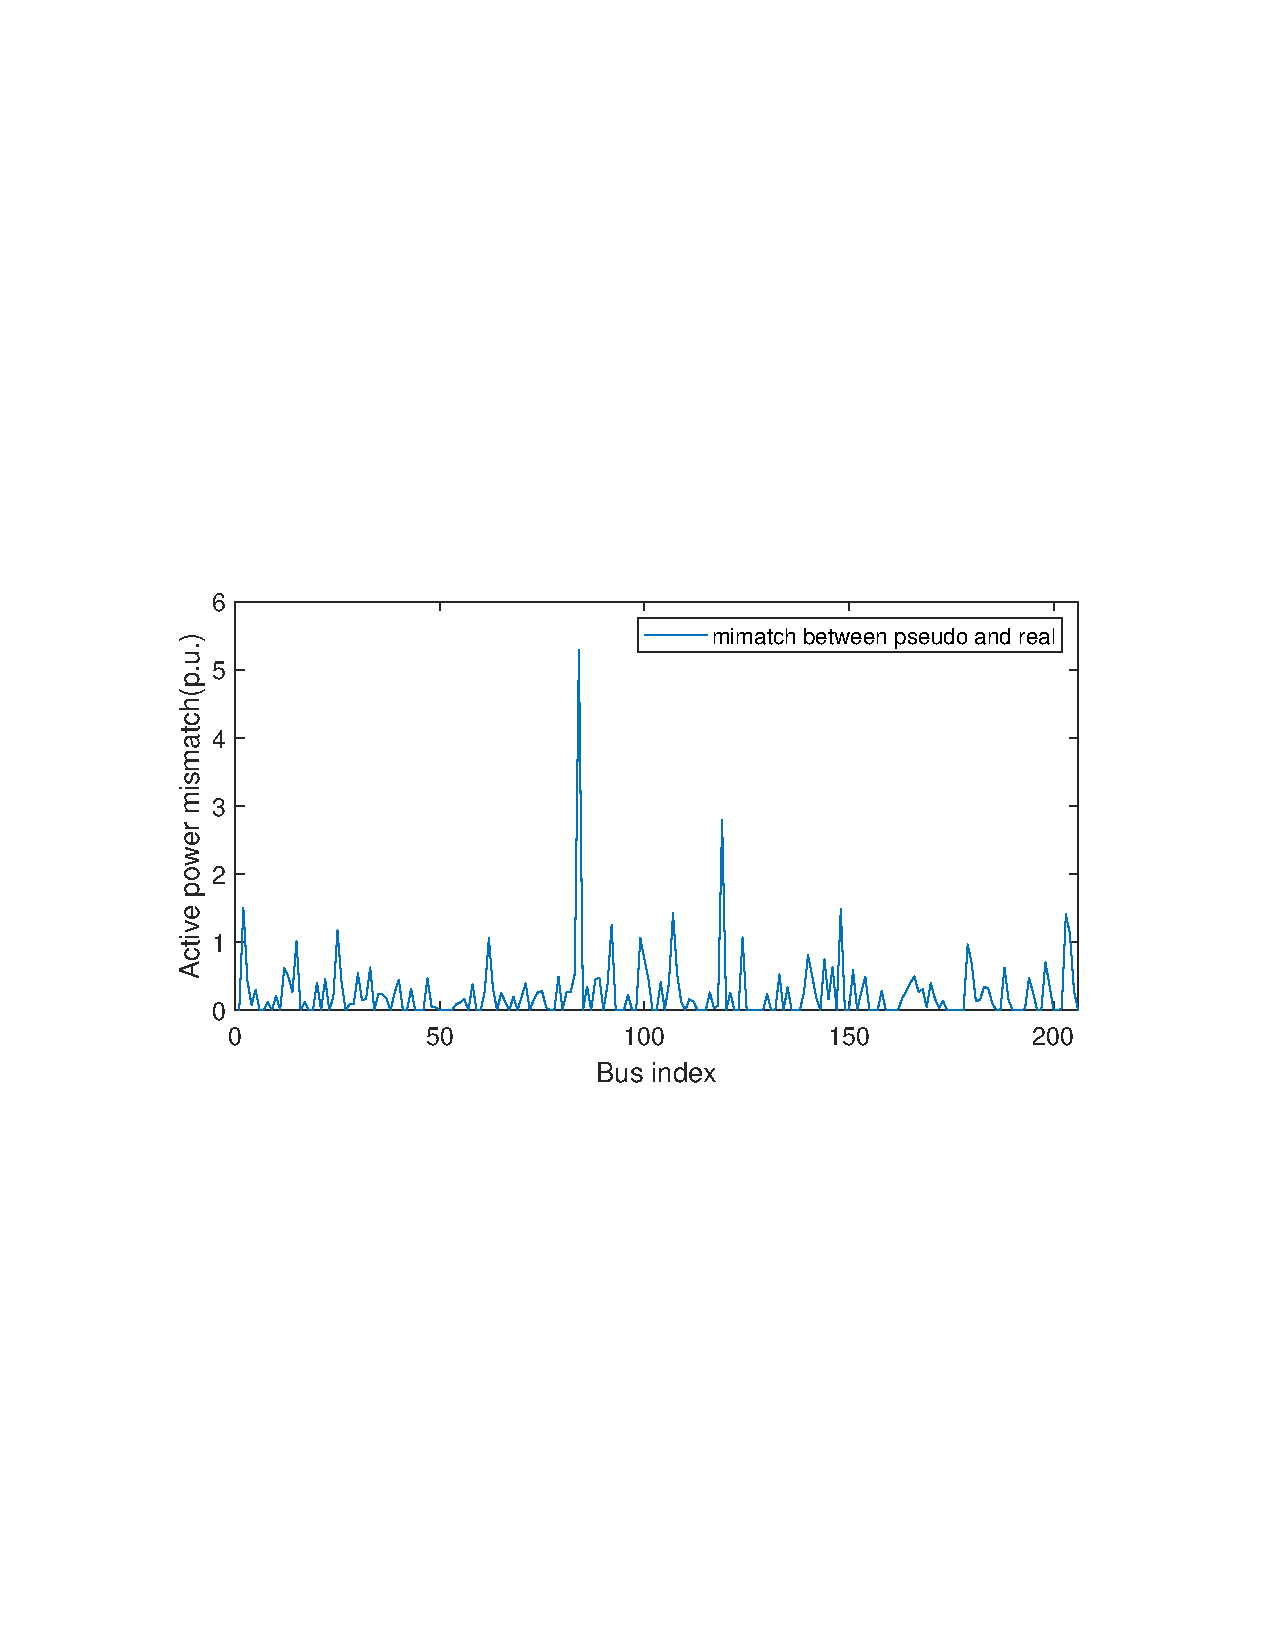
\includegraphics[ height=7cm, width=12cm]{figures/mismatch_psu_real.pdf}
        \caption{Total active power injection mismatch at each bus} 
        \label{fig:active power injection mismatch at each bus}
    \end{figure}
Even though the proposed pseudo-measurements generation method is based on the assumption that the total energy consumption at each node is known, there is still some total energy consumption mismatch between pseudo measurements and real measurement at the bus with a pseudo active power injection, as shown in Figure \ref{fig:active power injection mismatch at each bus}. The x-axis is the index of the 206 buses and the y-axis is the absolute mismatch between the real and pseudo measurements of 96 time steps. Notice that, obviously, there is no mismatch at with a real or virtual measurement. The reason why there is a mismatch at the pseudo measurement buses is that transmission losses are neglected in Equation \ref{eq:pseu_con}. As a result, the total active power consumption mismatch for all 206 buses depicted in Figure \ref{fig:active power injection mismatch at each bus} should be equal to the total active power losses during that day \cite{ghosh1997load}.